\documentclass[conference]{IEEEtran}
\usepackage{graphicx,times,amsmath,algorithm,caption, subcaption,nicefrac,bm}
\usepackage{multicol}
\usepackage[noend]{algpseudocode}
\usepackage{mathtools}
\usepackage{bbm}
\usepackage{amssymb}

\pdfminorversion=3

\newcommand{\defeq}{\vcentcolon=}
\newcommand{\eqdef}{=\vcentcolon}
\newcommand{\mathsc}[1]{{\normalfont\textsc{#1}}}
\newcommand{\argmax}{\operatornamewithlimits{argmax}}
\DeclareMathOperator*{\argmin}{arg\,min}
% correct bad hyphenation here
\hyphenation{op-tical net-works semi-conduc-tor}
% % \usepackage[table]{xcolor}

\DeclareMathOperator{\dis}{d}
\DeclarePairedDelimiter{\ceil}{\lceil}{\rceil}


\newcommand{\twopartdef}[4]
{
	\left\{
		\begin{array}{ll}
			#1 & \mbox{if } #2 \\
			#3 & \mbox{if } #4
		\end{array}
	\right.
}

\IEEEoverridecommandlockouts

\begin{document}

% Paper title: keep the \ \\ \LARGE\bf in it to leave enough margin.
\title{\ \\ \LARGE\bf Rolling Horizon methods for Games with Continuous Actions } 
% TODO - better title

\author{Samuel A. Roberts, Spyridon Samothrakis, Diego Perez, Simon M. Lucas}

% Uncomment out the following line for invited papers
%\specialpapernotice{(Invited Paper)}

% Make the title area
\maketitle


\begin{abstract}
It is often the case that games have continuous dynamics and allow for continuous actions. For larger games with complicated dynamics, having agents learn offline behaviours is a daunting task. On the other hand, provided a forward model is available, one might try to spread the cost of search in a rolling horizon fashion (e.g. as in example MCTS). In this paper we compare HOLOP, an open loop planning algorithm and a version evolutionary planning using CMA-ES. He show that rolling horizon CMA-ES outperforms HOLOP in two classic benchmark problems (Cart Balancing and <problem name> ) and Lunar Lander, a classic arcade game. We conclude that off-the-shelf evolutionary algorithms can be used successfully in a rolling horizon setting. 

\end{abstract}

% No keywords



\section{Introduction} \label{Introduction}
One of the most common uses of function optimisation is for solving control problems. If an agent has access to a generative model of the world (i.e. a simulator) in which it is going to act, a control problem becomes a search/optimisation problem, usually referred to as ``simulation based planning''. Recently, a family of algorithms, mostly known as Monte Carlo Tree Search (MCTS)~\cite{browne2012survey}, has been applied to planning problems of discrete states and actions with considerable success. The focus of these algorithms is to attack extremely large state spaces of perfect information games, where one can sample rewards from the state space easily (e.g. Computer Go~\cite{gelly2006modification}). With access to a generative model (from which one can easily sample) and perfect sensor information, the following procedure works well: the agent receives sensor information, formulates a plan of action, performs the first action of that plan, receives a new state, re-formulates a plan, acts again (using the first action of its plan),  ad infinitum.

The most important reason for continuous re-planning is the fact that most planning algorithms' computational complexity is linear (or worse) in the number of states, whereas the number of states increases exponentially at each time step. One thus hopes to perform an action that looks good now, act, and replan, effectively creating a smaller problem or a ``closer to action'' horizon. This kind of behaviour is known as rolling horizon, sample based or model predictive control/planning~\cite{chang2007simulation}. Most of these algorithms are not exact; at each time step, due to the large state space, planning takes place in a Monte Carlo fashion, with random ``rollouts'' (i.e. simulations) guiding the algorithm in a best first search manner. All this planning and replanning is computationally intensive, thus very efficient use of samples should be made.  In the case of discrete state and actions, bandit algorithms~\cite{auer2002finite} provided a formidable solution to this problem.
An example of exploiting this efficient sampling can be found in Samothrakis et al.~\cite{samothrakis2011fast} where a high-performance MCTS Pac-Man agent
was developed using only $50 - 300$ simulations per action (the game simulator requested an action
from the controller every 40ms).


Recently, algorithms stemming from, or at least partially inspired by, MCTS aiming at solving planning problems involving continuous states and actions have come to light. A typical such algorithm is Hierarchical Optimistic Open Loop Planing (HOLOP)~\cite{weinstein2012bandit}. HOLOP is based partially on a strong~\cite{hoo2011} real-valued optimisation algorithm called HOO (for ``Hierarchical Optimistic Optimisation''). In this paper two major contributions are made plus a smaller ``add-on''; the first contribution is the comparison of two versions of a very popular and strong evolutionary strategy: Covariance Matrix Adaptation Evolutionary Strategy (CMA-ES)~\cite{hansen2003reducing} and its Uncertainty Handling version UH-CMA-ES~\cite{hansen2009tec} with Truncated Hierarchical Optimistic Optimisation (T-HOO)~\cite{hoo2011} on the
Black Box Optimisation Problem (BBOP) benchmark suit~\cite{bbopnoisy}.  T-HOO is a faster version of HOO~\cite{hoo2011}, an algorithm reminiscent of Monte Carlo Tree Search. The experiments are conducted using similar conditions to those an agent would face if it was to solve planning problems. Our second contribution is to incorporate CMA-ES and UH-CMA-ES into three versions of an algorithm called EOLOP, for Evolutionary Open Loop Optimistic Planning.  This algorithm uses evolution instead of tree search for implementing sample-based control algorithms. We then proceed to test the algorithms proposed on noisy versions of standard reinforcement learning (RL)
benchmarks, namely the inverted pendulum and the double integrator problems. Our ``extra'' contribution is an add-on for evolutionary algorithms (transfered from HOLOP) that can help when the number of function evaluations is very small.

While evolution is commonly used to evolve a reactive neural network controller (in a process commonly called neuro-evolution) for these and other RL problems,
it should be noted that evolution is being applied in a very different way here. In this paper, evolution is applied to perform each action given the current state.  This approach can only be applied when a generative
model is available, but has the advantage of offering immediate good performance without any
prior learning.  The disadvantage, compared to neuro-evolution, is that every action performed requires
CPU time for the simulations.  This is described in more detail in section \ref{Planning}.

The rest of this paper is structured as follows.  Section \ref{Optimisation} discusses the relevant base algorithms that are going to be used in this paper, ((Truncated) Hierarchical Online Optimisation~\cite{hoo2011} and CMA-ES~\cite{hansen2003reducing}).
Section~\ref{Planning} explains why and how the above algorithms can be used in the context of planning. Section \ref{evo} describes how one can incorporate evolution into this, making this our main contribution section from an algorithmic standpoint. In Section \ref{Methodology} the experimental setup is described. In Section~\ref{sec:Experiments} a number of experiments are portrayed and analysed.  These form the bulk of this paper's contribution. We conclude with a short discussion in Section \ref{Conclusion}.


% TODO - actually determine what the core essence of what it is we're doing here before writing the introduction

\section{Motivation}



\subsection{Solving Continuous Problems with Continuous Actions} % this title is awful and it needs changing

Previous research into using MCTS to provide solutions for continuous physics-based problems have examined cases such as the Physical Travelling Salesman Problem \cite{perez14}. Within these continuous contexts, discrete actions have proven to be quite effective, especially with use of macro-actions and some degree of higher level planning \cite{powley12}.  % this section seems clunky

{\itshape Lunar Lander} is an excellent test case to study for many reasons, due to its inherently multi-objective nature. With the objectives to both land quickly while also minimising velocity changes, which cost fuel which must be conserved, it has been an interesting scenario to examine the properties and constraints imposed just by the environment alone. While there have been attempts to solve this deceptively complex problem before using discrete macro-actions \cite{roberts13}, in this paper the problem is being approached as one that can be better solved with continuous actions.

\section{Planning}  \label{Planning}
In this section a formalised version of planing will be presented and an explanation provided on how the algorithms described in the previous section can be used to attack the problem.
\subsection{Markov Decision Processes}

The main decision theoretic abstraction for planning/control is the Markov Decision Process (MDP)~\cite{howard1960dynamic}. Formally,  an MDP is a tuple $\langle S,A,T,R,\gamma\rangle$, where:

\begin{itemize}
\item $S$ is a set of states, $s \in S$, where $s_j^t$ is state $j$ at time $t$ and $s'_j$ is the state j at time $t+1$.
\item $A$ is a set of actions, each action named $a_j$.
\item  $T:S \times \S \times  A  \rightarrow [0,1]$ is the probability of moving from state $s$ to state $s'$  after action $a \in A$ has taken place. $T(s'|s,a)$ denotes this probability.
\item  $R:S \rightarrow \Re$, $R(s)$ is a reward function at each state.
\item $\gamma$, a discount factor.
\end{itemize}

The MDP defines a single agent environment, fully observable to the agent. In an MDP, the Markov property holds (hence the name), which means that all the information an agent needs in order to act is embedded in the current state.
A possible route of action an agent might take is known as the \textit{policy} $\pi$. A policy is a probabilistic mapping between state and actions, $\pi:S \times A \rightarrow [0,1]$, thus $\pi(s,a) \in [0,1]$,  $\sum_{a\in A}{\pi(s,a)} = 1$. The set of all policies is denoted as $\Pi$. The goal of an agent in an MDP environment is to maximise its long term value $V(\pi,s_0) = R(s) + \sum\limits_{s\in S}\sum\limits_{a\in A} \gamma \pi(s,a)T(s^\prime|s,a)  V(\pi,s^\prime) $, by assigning the probability of actions to take at each state.




\begin{figure}[ht]
  \centering
  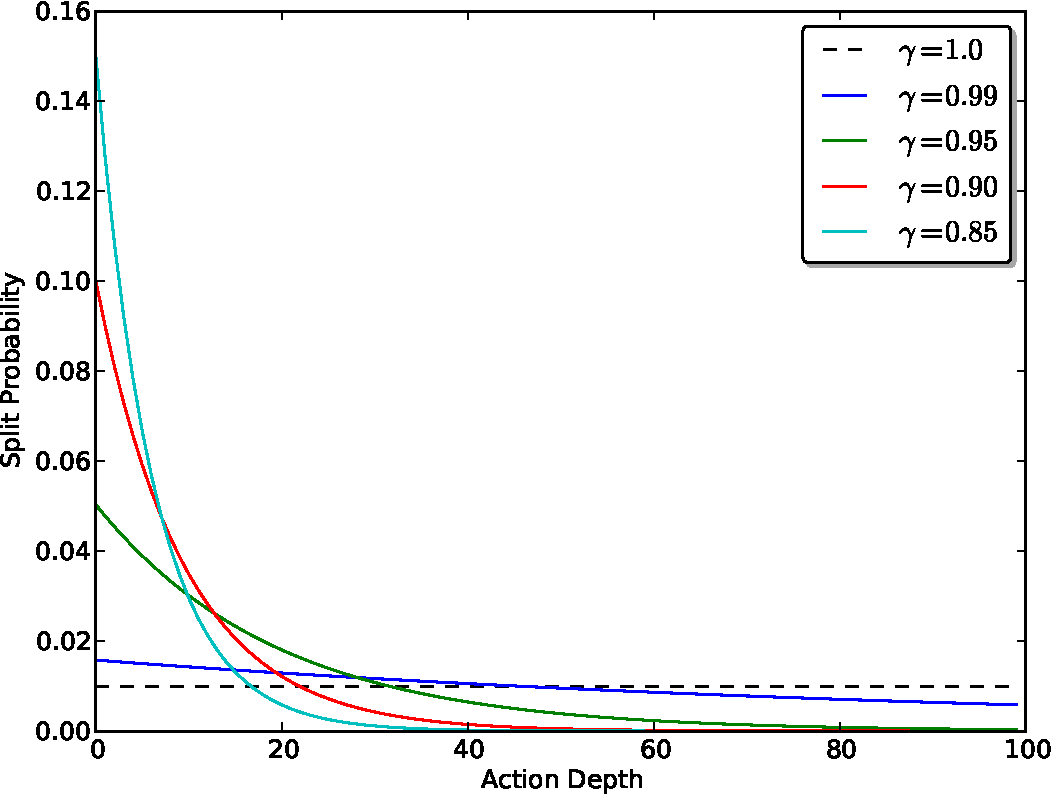
\includegraphics[width=0.45\textwidth]{graphics/gamma-crop.pdf}
  \caption{Examples of how rewards are affected by $\gamma$.}
  \label{fig:gamma}
\end{figure}


\subsection{Taxonomy of Planning Algorithms}
The terminology of Chang~\cite{chang2007simulation} is followed when trying to classify planning algorithms. If the policy $\pi:S \times A \rightarrow [0,1]$ is followed, what is known as ``closed loop'' planning takes place. The agent takes an action, senses its environment, takes another action etc. An alternative to closed-loop planning, ``open-loop'' planning, requires defining time. An agent sees a ``time'' when it's about to act instead of a state, i.e it doesn't have access to $s_t$, but just $t$. An open loop policy (or plan or control) is when an agent learns a policy with the form $\pi_o:S \times \mathcal{T} \rightarrow [0,1]$, where  $\mathcal{T}$ is an ordered set of time steps. Thus, an agent takes actions irrespective of the current state it is in. Intuitively this means that a sequence of actions is formed by the agent and the agent will take these actions in sequence (e.g. $(a_1,a_2,a_3,a_4,a_5,a_6,\dots,a_n)$). Obviously this is not optimal\footnote{Not optimal in the general case. It is optimal under the condition that the MDP is deterministic, i.e. each action leads to one specific state with probability one, and everything else has a probability zero}, although sometimes is much easier to do.


Another point of interest is planning, and when it happens. In open loop planning (and what is usually termed ``planning'' without any further qualifications), an agent forms a plan once and follows it until the end.

If the agent replans at every step, discarding or augmenting the plan received from previous steps, it is known as ``rolling horizon'' planning. The idea here is that, if the agent can plan as well as possible up to a  certain point, it can perform an action, move the planning horizon one step forward and replan. For example, Monte Carlo Tree Search for infinite MDPs can be seen as an approximate rolling horizon planning version of $TD(1)$\cite{silver2009reinforcement}.  The term ``Simulation based'' is used when the planning happens for an MDP that has a tree like structure and rewards are only visible at the end of the tree, a situation common in many games.

When learning how to act using a generative model, one can make a third distinction as to the type of sets represented by $A$ and $S$. In this paper the focus is on an $A$ and $S$ that come from a metric space. This means  that both sets' elements define a notion of distance and, for all practical purposes, have an infinite amount of elements. More specifically, both sets are drawn from a bounded set of real numbers, $\Re^n$.

Since an open loop policy is now a real-valued vector of actions, algorithms like T-HOO and CMA-ES can be used to find such a policy. Hence the title of this paper:  Rolling Horizon Open-loop Policy Evolutionary Learning. To the best of our knowledge this is the first time evolution has been used in such a setting. There are examples of closed loop rolling horizon papers, but these are beyond the scope of this article~\cite{xiang2012differential,samothrakis2010planning}.



\subsection{Planning using a Generative Model}

The Markov Decision Process simply describes an environment alongside the rewards that said environment provides to an agent. A problem central to Artificial Intelligence is what actions an agent must take to maximise its long term reward. The most basic assumption one can make is that the agent knows nothing about the environment. In this case the agent gets thrown into the environment and interacts (``trains'') for some time. After the training is complete, the agent should be able to act intelligently (presumably with some success).

Another approach one can take is to assume that the agent has a copy of the MDP in its ``mind'' and thus is able to plan accordingly. This is usually termed dynamic programming~\cite{sutton1998reinforcement}, however it cannot be used in the case of continuous states or actions without the use of a function approximator (FA) or some kind of discretization. Another approach, and one which has made a significant impact recently, arguably presented for the first time by Kearns~\cite{citeulike:1584916} and popularised mostly as Upper Confidence Bounds for Trees (UCT)~\cite{kocsis2006bandit}, is to use a generative model.

A generative model is nothing more than a simulator of future events. This is a less of a requirement than knowing the full model (which entails knowing the full function $T$), but still requires the agent to have some knowledge of the world. This category of algorithms, which are broadly termed ``Rolling Horizon'', has the following steps. From the current state, a number of simulations of possible futures is run by executing a set of action sequences (all of this in the ``mind'' of the agent). The simulations last for a certain number of steps (hence the ``rolling horizon'') or continue until an end state is encountered (i.e. when the MDP has ``absorbing'' states that cannot be acted from).

Once a satisfactory plan/policy has been estimated (or the agent runs out of time, iterations etc. ) it proceeds by executing the first action of the plan, thus moving to the next state. Once there, the agent performs the same sequence of ``mental'' actions, (i.e. plans and executes the first action), until some predefined stopping condition.  In this paper we will concern ourselves \textit{only} with this method of planning. What changes from method to method is how the plan is formed.

In standard UCT, a procedure similar to temporal difference learning is followed, where one learns the value of each state. An agent then forms a policy by choosing a value greedily. In our case, because our state space has continuous states and actions, this is impossible without the use of a function approximator (or an infinite discretization of space), which is not attempted here. What is attempted though is to learn the policy function directly without reference to state, while planning continuously from the current state. So while the agent forms open-loop plans at each clock tick, in reality it is executing a closed-loop policy. While the strategy is not provably optimal, it can work well in practice~\cite{weinstein2012bandit}. This will be seen by our experimental results (see Section \ref{sec:Experiments}).



\begin{algorithm}[!ht]
\caption{Rolling Horizon Open Loop Planning}\label{algo:ooop}
\begin{algorithmic}

\State 	\textbf{define external function} $\mathsc{FindOpenLoopPlan} (depth) $ \Comment{Try to find the optimal policy. You can use either evolution or HOO here}


	\Procedure{$\mathsc{OOOP}$} {}
		\While{$\mathit{True}$}
		    \State $a \gets \mathsc{FindOpenLoopPlan}(depth)[0]$ \Comment{Execute first action of the policy}
		    \State $s \sim T(s'|s,a)$ \Comment{Stop only at an absorbing state}
		\EndWhile
		\State
	\EndProcedure



\end{algorithmic}
\end{algorithm}


\section{Methodology}

\subsection{Simple Planning Benchmarking Problems}

% % \todo[inline]{Simon to do this}.




For direct comparison with recent work on sample based planning using trees, in particular
Weinstein and Littman~\cite{weinstein2012bandit} and Pazis and Lagoudakis \cite{PazisBAS},
we used the same problems: double integrator, and inverted pendulum.  The basic
experimental setup followed Weinstein and Littman~\cite{weinstein2012bandit}
and Pazis and Lagoudakis \cite{PazisBAS}
closely, except that they used a fixed noise level for each experiment whereas we varied the
noise level to explore how performance was affected.

Both problems are modelled
using continuous state discrete time simulations.  In each case the desired
acceleration is corrupted by additive uniform random noise
before being limited within the specified range.  The noise levels are described in the next section.


\subsubsection{Double Integrator}

The double integrator problem is to control a mass along a single dimension.  The state space
is 2-dimensional, consisting of $(p,v)$ where $p$ is position and $v$ is velocity.
The goal is to change the state from $(1,0)$ to $(0,0)$.  Both position and velocity
are clamped to be within the range $-2$ to $+2$.  At each time step the controller selects
the desired acceleration $a'$, which then is noise corrupted and range limited between $-1.5N$ to $+1.5$N to yield the
applied acceleration $a$.

Euler integration is then used to update the position and velocity, given the time step $\delta_t$:

\begin{eqnarray}
v_{t+\delta_t} & = & v_{t} + a \delta_t \\
p_{t+\delta_t} & = & p_{t} + v_{t+\delta_t} \delta_t
\end{eqnarray}

At each time step the reward $r$ is:
\begin{equation}
 r = -(p^2 + a^2)
\end{equation}

The problem becomes harder as the time interval $\delta_t$ at %word missing?
each action is applied increases,
and following Pazis and Lagoudakis we set $(\delta_t = 0.5s)$.

% \begin{equation}
% R = -(p^2 + a^2)
% \end{equation}

\subsubsection{Inverted Pendulum}

The inverted pendulum problem is also known as the pole balancing
or cart-pole problem.  The goal is to keep the pendulum / pole as upright and as still as possible.
This is achieved by accelerating the cart which affects the freely pivoted pendulum.

In this instance of the problem the controller only sees a two dimensional
state space, consisting of the
angle $\theta$ that the inverted pendulum deviates from the vertical, and the angular velocity
of the pendulum $\dot{\theta}$.
The controller selects the desired angular force $F$,
which is then corrupted by additive uniform random noise and limited in the range $-50N$ to $+50$N
so as to yield the applied angular force $u$.  The angular acceleration $\ddot{\theta}$ is then calculated
as follows:

\begin{equation}
\ddot{\theta} = \frac{g sin(\theta) - \alpha m l (\dot{\theta})^2 sin(2 \theta) / 2 - \alpha cos(\theta) u}
                     {4l/3 - \alpha m l  cos^2(\theta)}
\end{equation}

where $g$ is the acceleration due to gravity
$(g = 9.8ms^{-2})$,
$m$ is the mass of the pendulum
$(m = 2kg)$, $(\alpha = 1 / (m + M))$, $M$ is the mass of the cart
$(M = 8kg)$ and $l$ is the length of the pendulum $(l = 0.5m)$.
The time interval $\delta_t$ was set to $0.1s$: i.e.\ the simulation is
updated 10 times per second:

\begin{eqnarray}
\dot{\theta}_{t+\delta_t} & = &  \dot{\theta}_{t} + \ddot{\theta} \delta_t \\
\theta_{t+\delta_t}  & = & \theta_{t} + \dot{\theta}_{t+\delta_t} \delta_t
\end{eqnarray}

At each timestep the reward $r$ punishes deviation from the vertical, high speed, and high force:
\begin{equation}
r = -((2 \theta / \pi)^2 + \dot{\theta}^2 + (F / 50)^2 )
\label{eq:rew:t}
\end{equation}


\subsection{Environment and Physics}

% this is a heavily cut down rewritten version of the physics described in sam's 2013 cig paper
% more detail will be added depending on if it is appropriate or not

\subsubsection{Environmental Properties}

The properties of the base environment of {\itshape Lunar Lander} are that it is frictionless, and that it is a two-dimensional plane with horizontal wrapping. This can also be conceptualised as a cylinder. Anything that passes from the left edge of the playing field moves to the right instantaneously, and vice versa.

The other feature of note is the jagged landscape, a simplistic representation of the noisy, crater-filled lunar landscape the game represents. This landscape is constructed as a series of line segments, with each vertex of the jagged landscape being distributed equally horizontally, and randomly vertically. % unclear?

% TODO: DIAGRAM - jagged lunar landscape might be useful (reuse of old one probably not sufficient)

% not sure how much detail should be gone into here? should just cite generation equations from old paper or copy over??

Each vertex of this landscape is generated sequentially. % INCOMPLETE due to uncertainty listed above


\subsubsection{Spaceship Physics}

The spaceship within this game world is modelled as an a circular mass with some basic physical properties, such as a position within the game world $\boldsymbol {s}$, a velocity $\boldsymbol {v}$, an orientation $\theta$, an angular velocity $\omega$ and a radius of a bounding sphere $r$ used for collision detection with the landscape.

This collision detection method is based on the lowest point of the spaceship's bounding circle coming into intersection with the highest point of the landscape for the line perpendicular between the ship and the bottom of the playing field, as can be seen in Figure \ref{fig:diagram_landscapepoint}.

% this needs a diagram for clarity: reuse the old one? reusing it temporarily
\begin{figure}[hbtp]
\centering
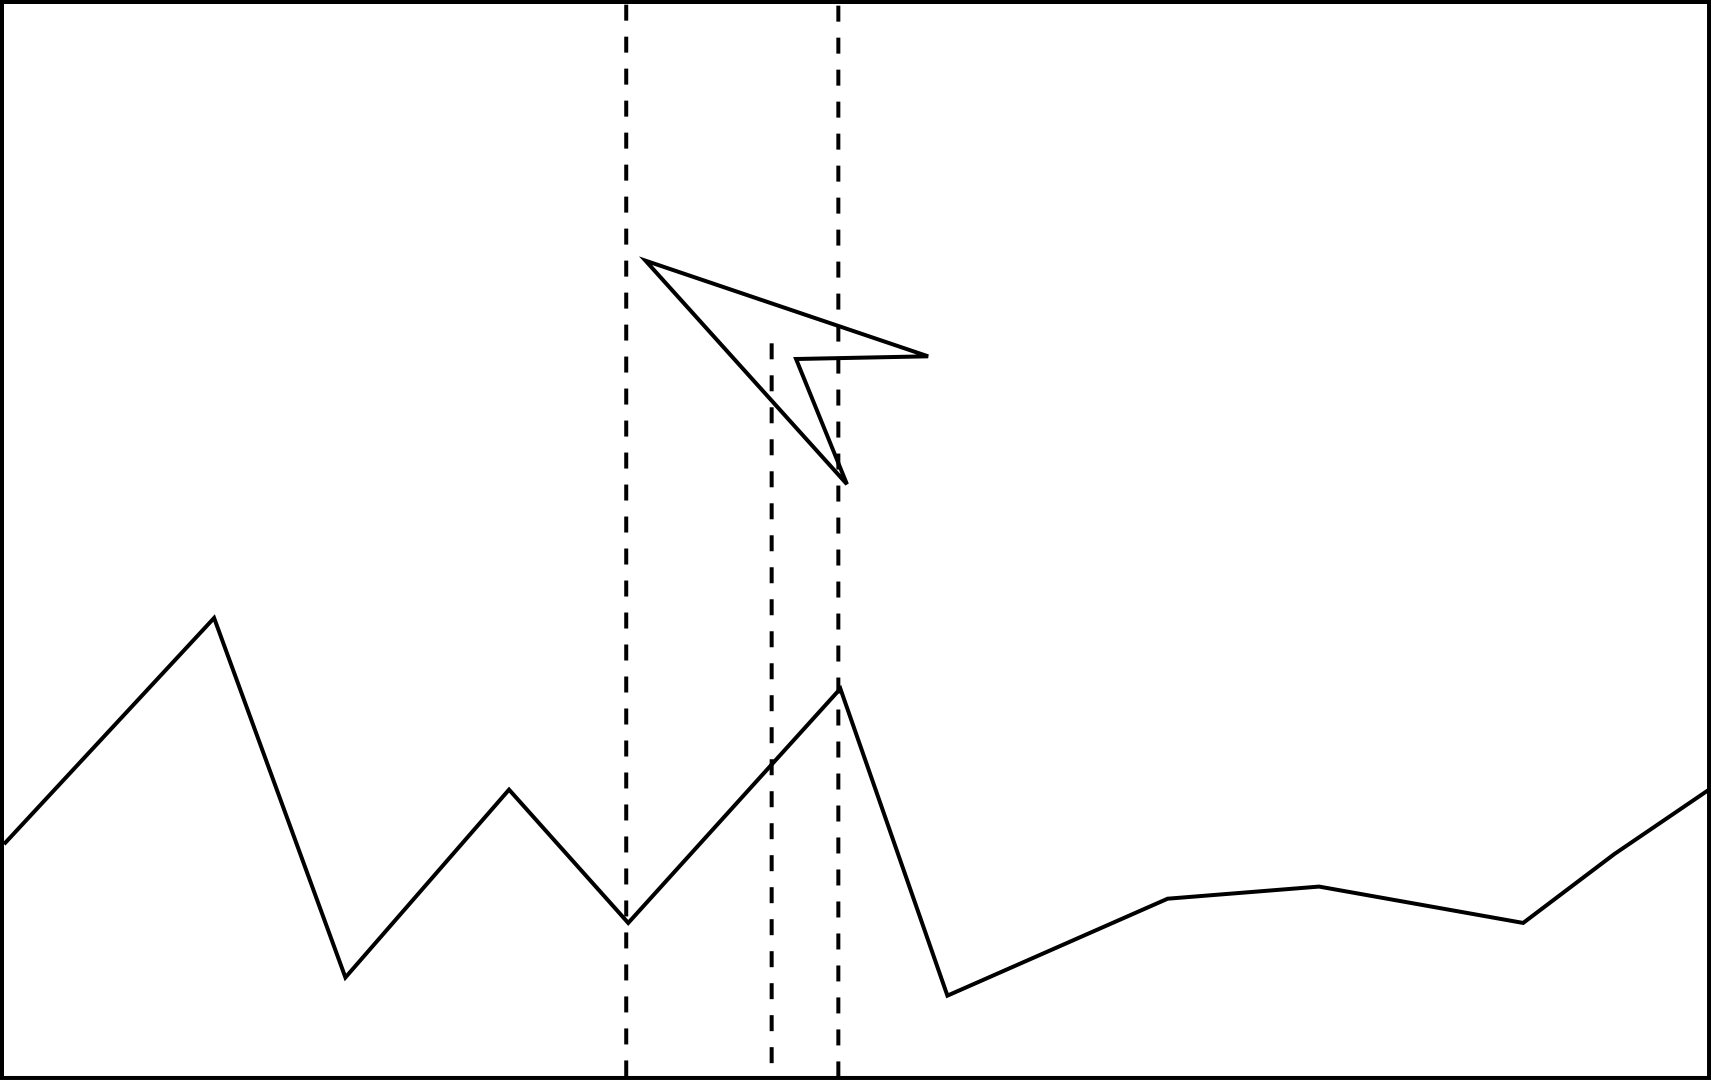
\includegraphics[scale=0.4]{graphics/landscapepoint}
\caption{The point closest to the spaceship on the landscape lies in between two of the defined vertices of the landscape, and requires interpolation to calculate the y co-ordinate from the x co-ordinate of the ship.}
\label{fig:diagram_landscapepoint}
\end{figure}

As the landscape is stored as a series of line segments, interpolation must be used in the event the ship is not perfectly aligned with one of the landscape axes. The point that lies on the line segment that the ship is being checked against is calculated through simple linear interpolation based on which two vertices the ship is horizontally closest to. For the ship's centre $\boldsymbol {s}$, the left nearest landscape vertex $\boldsymbol {p}^{l}$ and the right nearest landscape vertex $\boldsymbol {p}^{r}$, the point of collision $\boldsymbol {p}^{c}$ against the landscape is calculated as 

% does this constitute self-plaigarism???

\begin{equation}
\boldsymbol {p}_{x}^{c} = \boldsymbol {s}_{x}
\boldsymbol {p}_{y}^{c} = \boldsymbol {p}_{y}^{l} + v(\boldsymbol {p}_{y}^{r} - \boldsymbol {p}_{y}^{l})
\end{equation}

where $v$ is a value between $0$ to $1$ used for interpolation, and can be calculated as follows.

\begin{equation}
v = \frac{ {\boldsymbol {s}_{x} - \boldsymbol {p}_{x}^{l}}}{ {\boldsymbol {p}_{x}^{r} - \boldsymbol {p}_{x}^{l}} }
\end{equation}

Collision is then true if the following statement is true:

\begin{equation}
\boldsymbol {s}_{y} + r \geq \boldsymbol {p}^{c}_{y}
\end{equation}

The ship colliding with the landscape constitutes the end of the {\itshape Lunar Lander} game. The conditions surrounding this collision, including speed, orientation of the ship, and fuel used, constitute whether the nature of the collision is a success or a failure.


\subsection{Continuous Action MCTS} % this can be renamed something much better presumably

\subsubsection{Heuristic} % this too

% TODO - meeting or discussion might be good to be entirely certain on what's going on in the code
% DISCUSS IN MEETING: use of a two-stage approach: might be good to mention this?? temporary holdover?????

\section{Results}




\begin{figure*}[ht]
  %\centering



  \centering
        \begin{subfigure}[b]{0.32\textwidth}
                \centering
                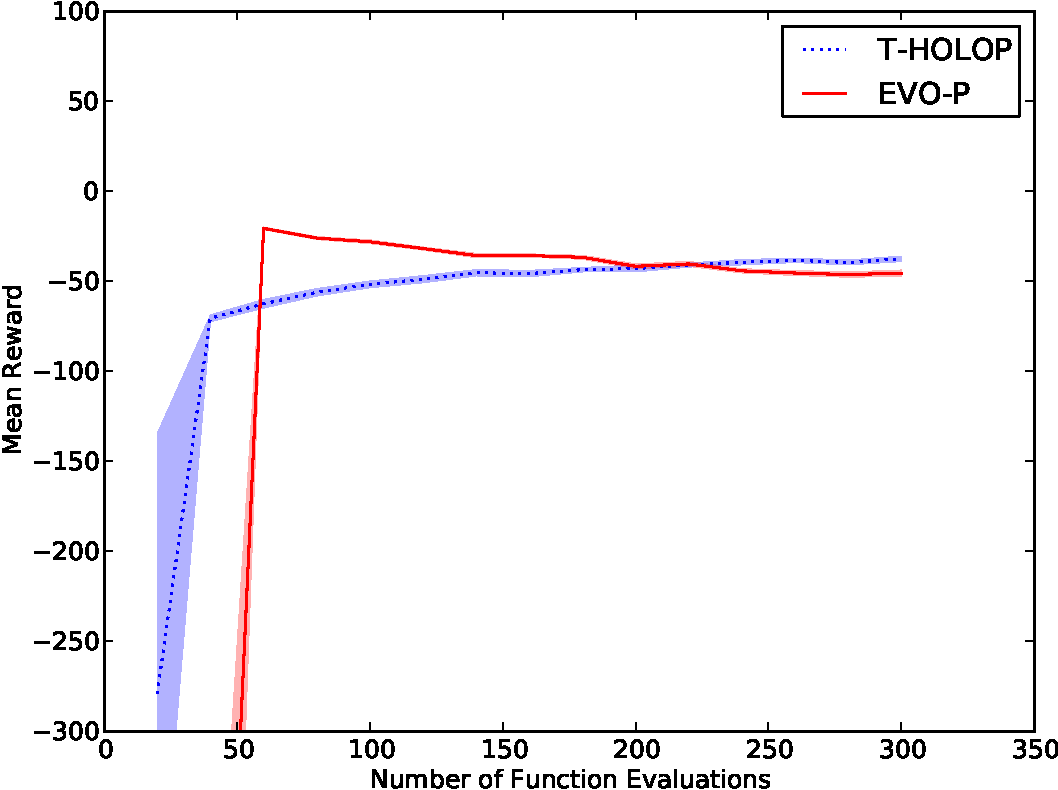
\includegraphics[width=1.0\textwidth]{graphics/online-IP-crop.pdf}
                \caption{Scores for a noise level of $l=1$ under variable function evaluations.\vspace{0.14in} }
                \label{fig:IP}
        \end{subfigure}   \begin{subfigure}[b]{0.32\textwidth}
                \centering
                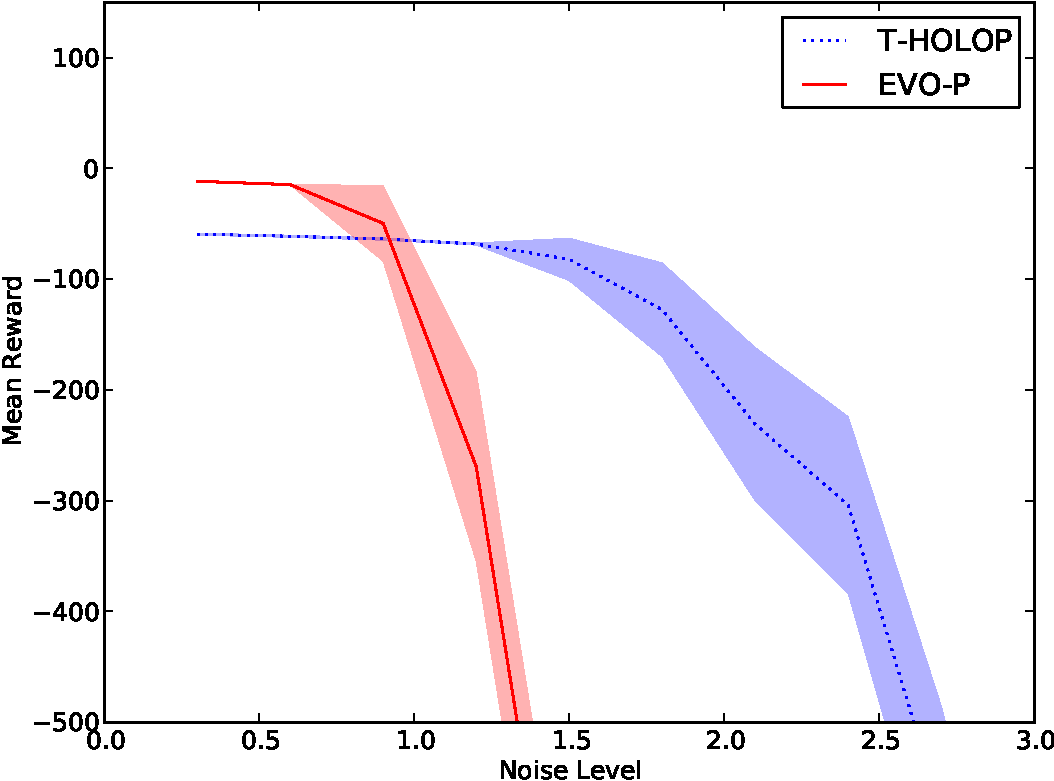
\includegraphics[width=1.0\textwidth]{graphics/online-noise-IP_50-crop.pdf}
                \caption{Scores for 50 iterations under variable noise level $l$. Notice how UH-EOLOP fails to balance the pole.}
                \label{fig:IP-N-50}
        \end{subfigure}  \begin{subfigure}[b]{0.32\textwidth}
                \centering
                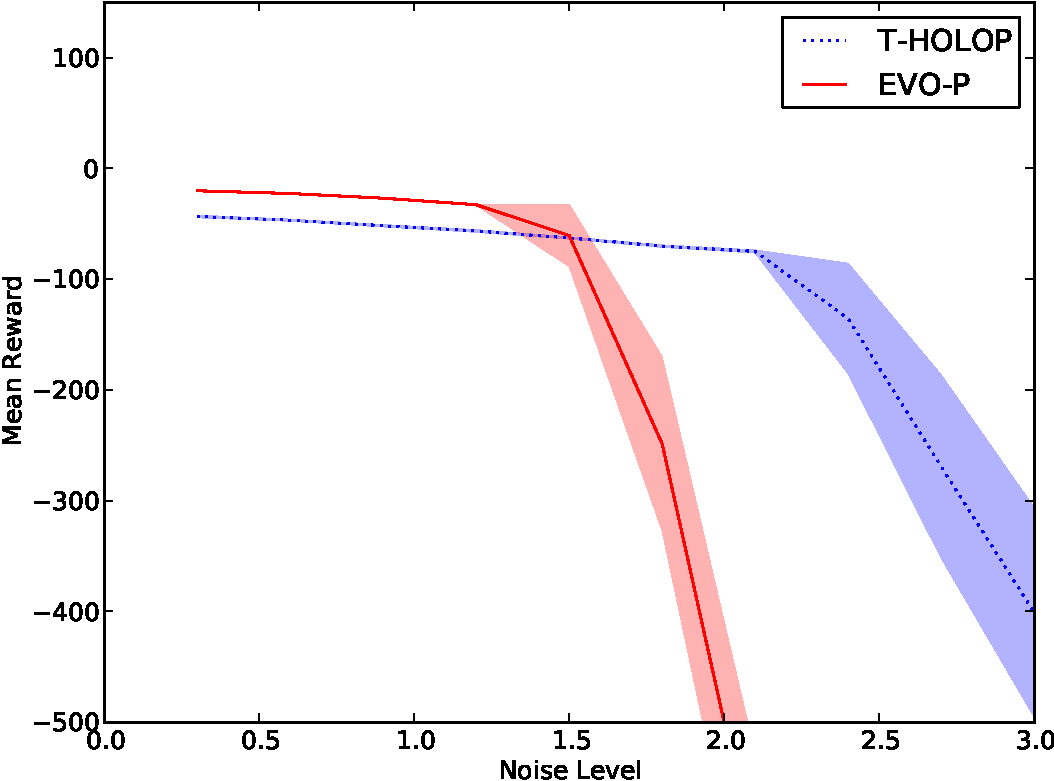
\includegraphics[width=1.0\textwidth]{graphics/online-noise-IP_100-crop.pdf}
                \caption{Score for 100 iterations under variable noise level $l$.\vspace{0.14in}}
                \label{fig:IP-N-100}
        \end{subfigure}%

         \caption{Performance of all algorithms in the Inverted Pendulum benchmark (error bars for the 95th percentile). Higher scores are better}
         \label{fig:IP-all}

\end{figure*}


        \begin{figure*}[ht]

        \begin{subfigure}[b]{0.32\textwidth}
                \centering
                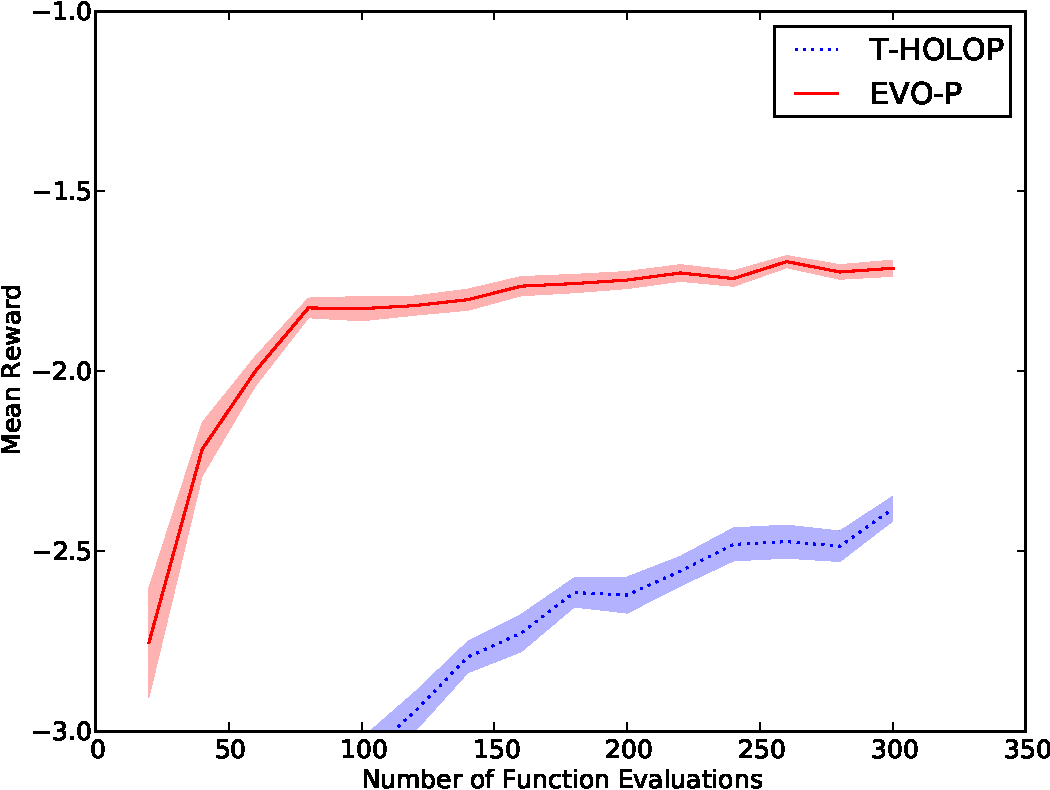
\includegraphics[width=1.0\textwidth]{graphics/online-DI-crop.pdf}
                \caption{Scores for a noise level of 1 under variable function evaluations.}
                \label{fig:DI}
        \end{subfigure}   \begin{subfigure}[b]{0.32\textwidth}
                \centering
                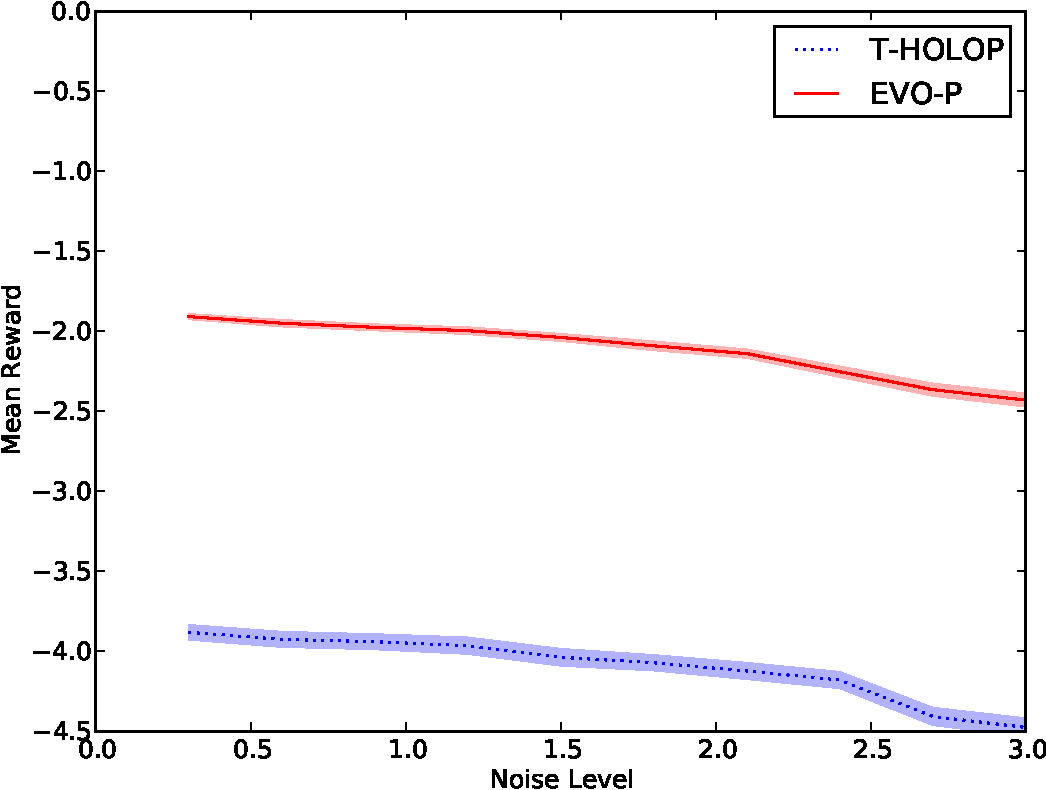
\includegraphics[width=1.0\textwidth]{graphics/online-noise-DI_50-crop.pdf}
                  \caption{Scores for 50 iterations under variable noise level $l$. }
                \label{fig:DI-N-50}
        \end{subfigure}   \begin{subfigure}[b]{0.32\textwidth}
                \centering
                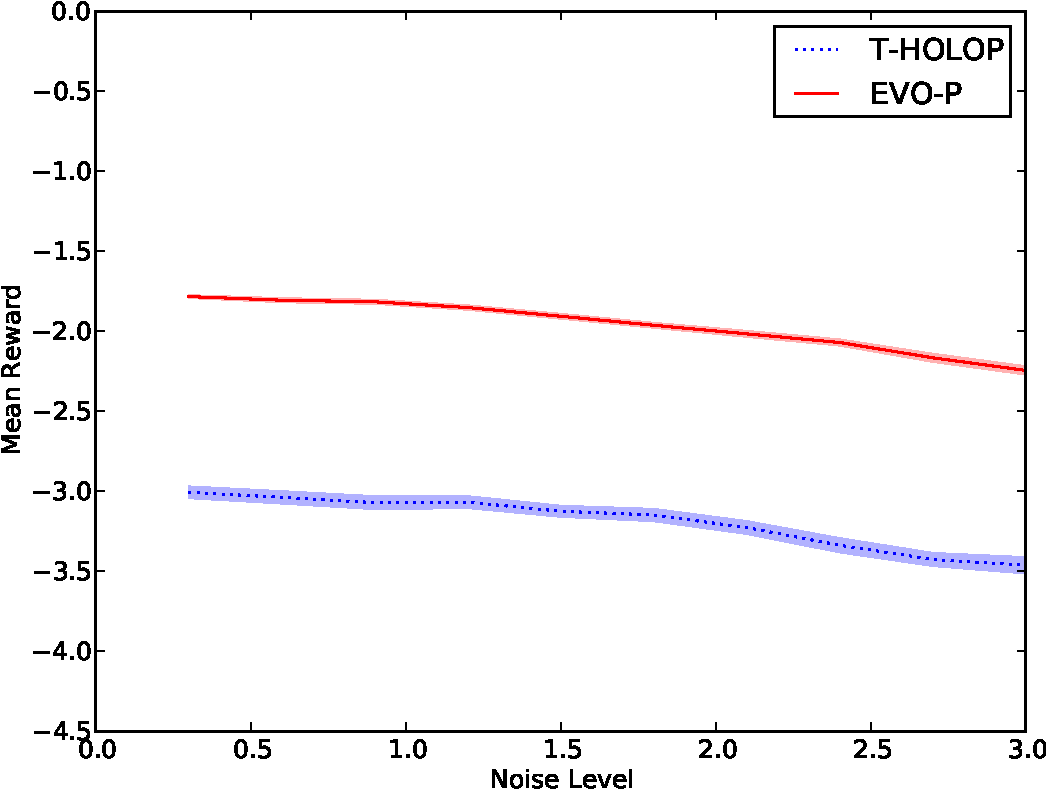
\includegraphics[width=1.0\textwidth]{graphics/online-noise-DI_100-crop.pdf}
                \caption{Score for 100 iterations an variable noise level $l$.}
                \label{fig:DI-N-100}
        \end{subfigure}

  \label{fig:DI-all}

       \caption{Performance of all algorithms in the Double Integrator benchmark (error bars for the 95th percentile). Higher scores are better}


\end{figure*}


\section{Conclusion}

% pending
% DISCUSS IN MEETING: this entire section
 
% Use \section* for the acknowledgments
\section*{Acknowledgements}
Samuel Roberts is supported by an EPSRC PhD Studentship.
% any other acknowledgements??

\bibliographystyle{IEEEtran}
\bibliography{lunarcontbib}
\end{document}